\documentclass[a4paper, 10.5pt, titlepage]{article}
\usepackage{fancyhdr}
\usepackage{graphicx}
\usepackage{imakeidx}
\usepackage{makeidx}
\usepackage{mathtools}
\usepackage[spanish]{babel}
\usepackage{eurosym}

% CODE C
\usepackage{amssymb}
\usepackage{listings}
\usepackage{xcolor}
\definecolor{textblue}{rgb}{.2,.2,.7}
\definecolor{textred}{rgb}{0.54,0,0}
\definecolor{textgreen}{rgb}{0,0.1,0}
\lstset{language=C, 
numbers=left, 
numberstyle=\tiny, 
stepnumber=1,
numbersep=5pt, 
tabsize=4,
basicstyle=\ttfamily,
keywordstyle=\color{textblue},
commentstyle=\color{textred},   
stringstyle=\color{textgreen},
frame=none,                    
columns=fullflexible,
keepspaces=true,
xleftmargin=\parindent,
showstringspaces=false}

\title{LaTeX}
\author{Alberto Fraile}
\date{2020}

\begin{document}

\maketitle
\tableofcontents
\newpage

\begin{section}{Estructura y desarrollo de un artículo}\end{section}

\begin{lstlisting}
    \documentclass[a4paper, 10pt, titlepage]{article}

    \usepackage{hyperref}
    \usepackage[utf8]{inputenc}
    \usepackage[spanish]{babel}
    \usepackage{graphicx}
    
    \title{Ejemplo}
    \author{Ejempla Ejemplez}
    \date{2020}
    

    \begin{document}

    \maketitle
    \tableofcontents
    
    \\ Nuevo parrafo

    \section{Nombre} 
    \section*{Sin Numeracion}

    \subsection{Nombre} 
    \subsection*{Sin Numeracion}

    \subsubsection{Nombre}

    \textbf{Negrita} \textit{Cursiva} \underline{Subrayado}
    
    \label{'Etiqueta'}
    \ref{'Etiqueta'}

    \begin{quote}
        \small <<Ejemplo de cita>>
    \end{quote}

    \begin{figure}[htp]
        \centering
        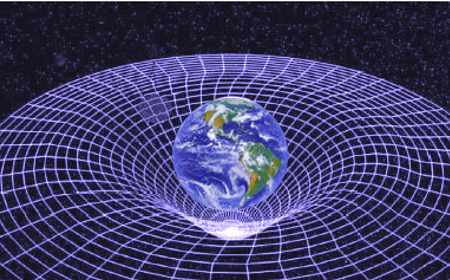
\includegraphics[width=0.8\textwidth]{imagen.jpeg}
        \caption{Descripcion de la fotografia}
        \label{imagenejemplo}
    \end{figure}

    \end{document}
\end{lstlisting}    

\newpage

\end{document}